% !TEX root = ../paper_zh.tex
\begingroup
\makeatletter
\setlength{\@fptop}{0pt}
\setlength{\@fpsep}{12pt}
\makeatother
\section{数据分布与补充视觉证据}
\label{sec:visual_details_zh}
\setcounter{figure}{0}
\renewcommand{\thefigure}{B.\arabic{figure}}

图~\ref{fig:dataset_details_zh} 报告逐场景数量和采集属性。
图~\ref{fig:additional_product_zh} 与图~\ref{fig:night_control_zh} 将正文案例扩展到电塔环绕序列
及夜间变焦/广角对照。所有可视化使用冻结的变换估计，裁剪范围与对应源记录一致。

\begin{figure}[!htbp]
\centering
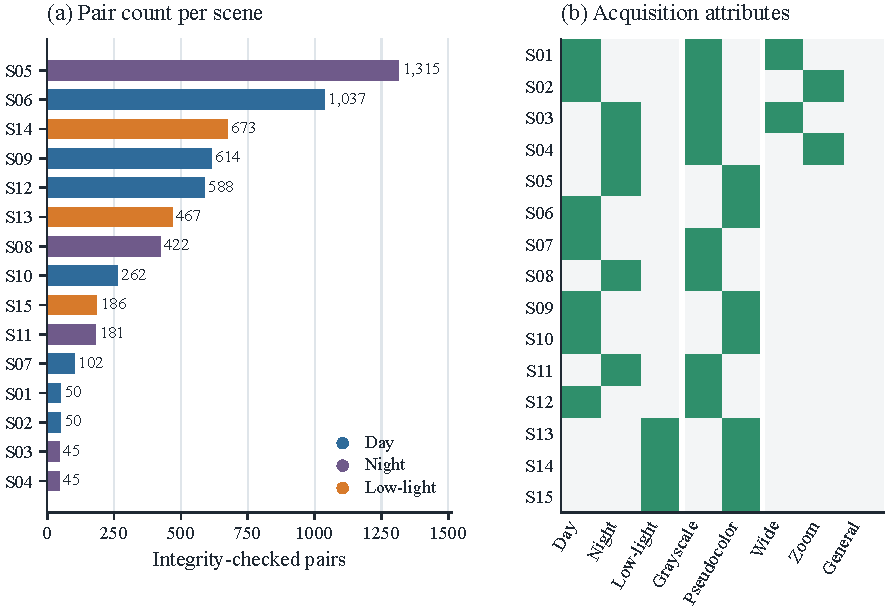
\includegraphics[width=\textwidth]{figures/fig02_dataset_details.pdf}
\caption{正式评测划分：（a）15 个场景的有效图像对数量；（b）采集属性。
（a）中的颜色表示光照条件，（b）中的填充单元格表示场景属性。}
\label{fig:dataset_details_zh}

\vspace{10pt}
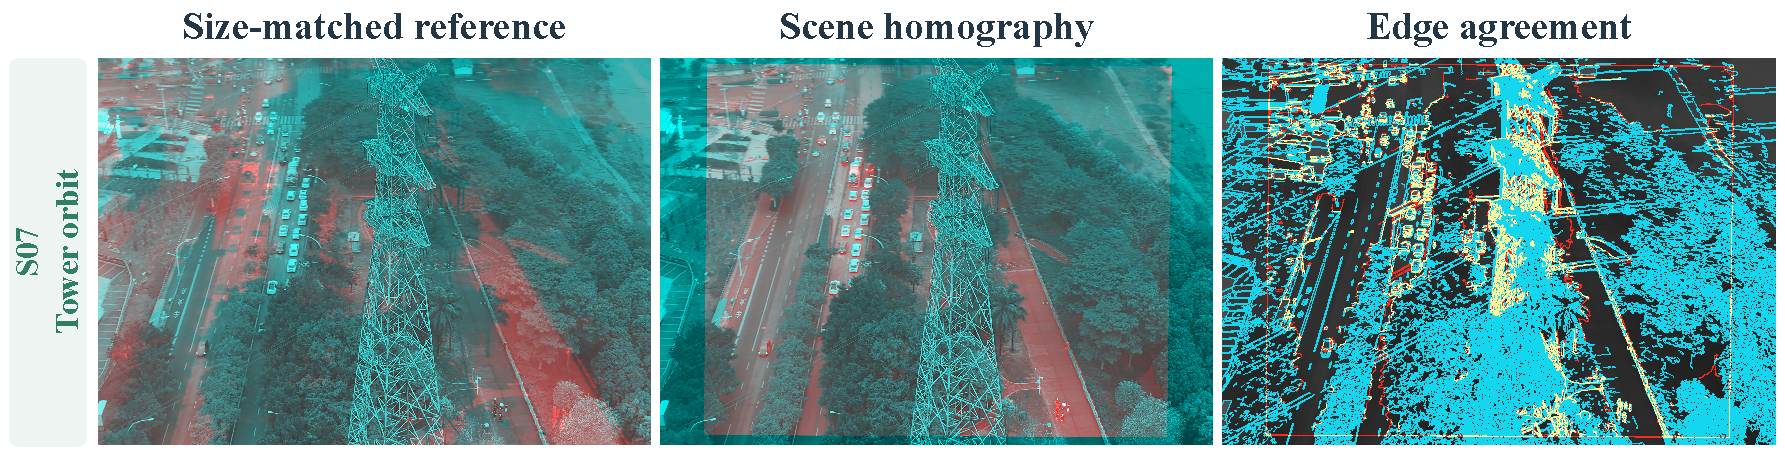
\includegraphics[width=\textwidth]{figures/fig06_additional_product.pdf}
\caption{S07 电塔环绕序列的补充规范产品。三个子图在同一显示裁剪范围内比较尺寸匹配参考、
场景单应性叠加和边缘一致性。}
\label{fig:additional_product_zh}
\end{figure}

图~\ref{fig:all_scene_qa_zh} 将全部场景投影到接受支撑与相对离群点空间。
参考线属于基线感知验证路径；完整规范决策还包含附录~\ref{sec:canonical_details_zh}
中定义的主路径与支撑要求。

\begin{figure}[!htbp]
\centering
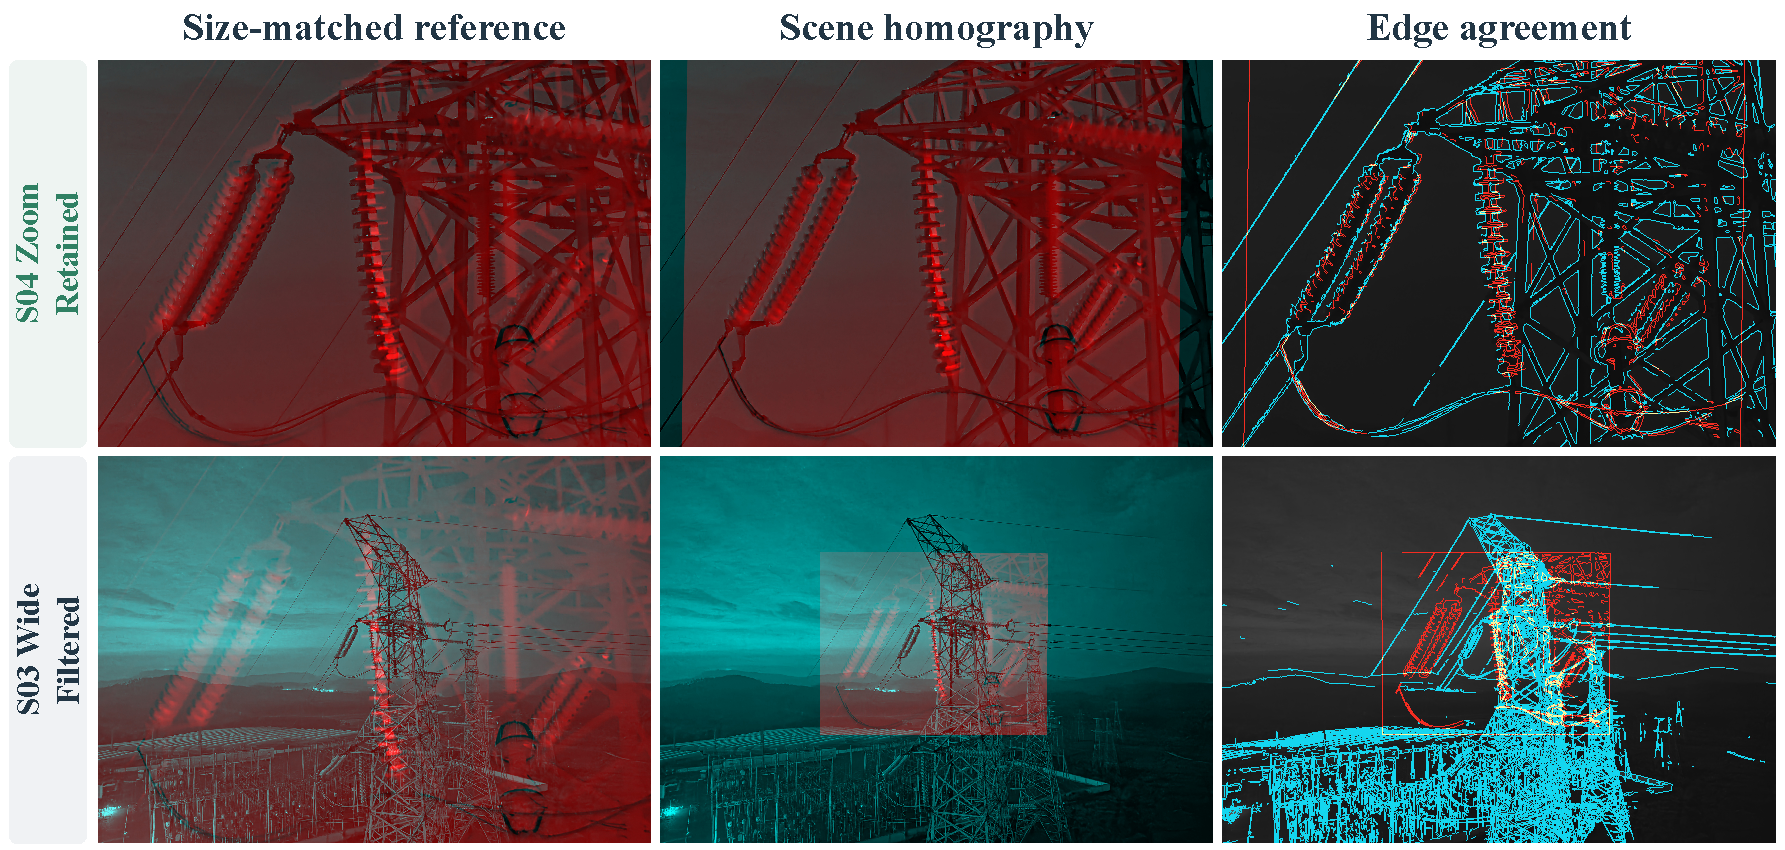
\includegraphics[width=\textwidth]{figures/fig07_night_control.pdf}
\caption{夜间变焦/广角对照。S04 被规范门控保留，S03 被 QA 过滤。
每行展示尺寸匹配参考、估计的场景单应性和边缘一致性。过滤场景的变换保留展示以供检查。}
\label{fig:night_control_zh}

\vspace{10pt}
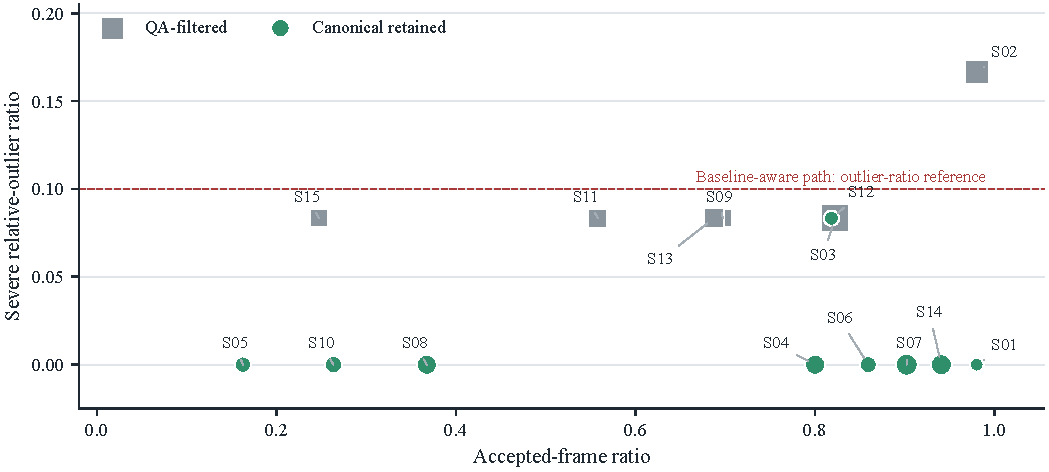
\includegraphics[width=\textwidth]{figures/fig07_qa_scatter.pdf}
\caption{全场景 QA 诊断。圆点为规范保留场景，方块为 QA 过滤场景；标记大小表示鲁棒剔除比例。
虚线表示基线感知路径中使用的 0.10 严重离群比例参考。}
\label{fig:all_scene_qa_zh}
\end{figure}
\FloatBarrier
\endgroup
